\chapter{Prosthesis and control} \label{prostheses}

A prosthesis is many things, for some users, it is to give a visual sense of having a complete set of limbs, where other prosthesis have some functionality built in, here is a short description of some that are on the market right now.

\paragraph{Aesthetics prosthesis}
This is a prosthesis that used to visually mimic the missing limb. they are mainly used so the user of prosthesis can feel as part of the society without having to answer, every curious gaze from bystanders. Aesthetics is often seen as a passive device, but the aesthetics prosthesis supports the user so the body weight is more uniform\cite{aesthetic}.  
\begin{figure}[H]
    \centering
    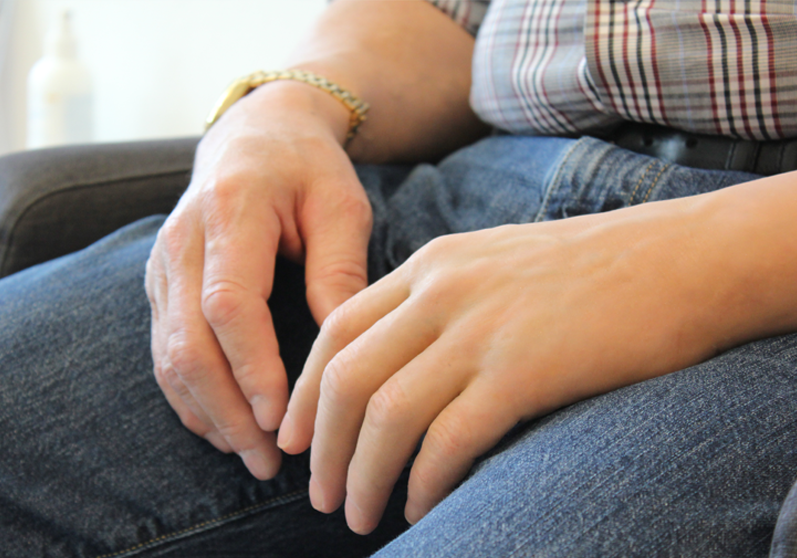
\includegraphics[width=10cm,height=7cm]{Figures/Contextual_figures/ProsthesesPics/aestikarm.png}
    \caption{Aesthetic arm prosthesis from Shava(left arm)\cite{aesthetic}.}
    \label{fig:aesthetic}
\end{figure}
\paragraph{Mechanical prosthesis}
A mechanical arm is made depending on the users amputation level, some are controlled with the elbow joint and some with the wrist and for high-level amputees such as shoulder disarticulation, the user moves the arm in position, with the other hand, if for instance a user wants to lift a box, the user manipulates the arm with the other hand, so it can grasp the box in collaboration, with the able hand. 
\begin{figure}[H]
    \centering
    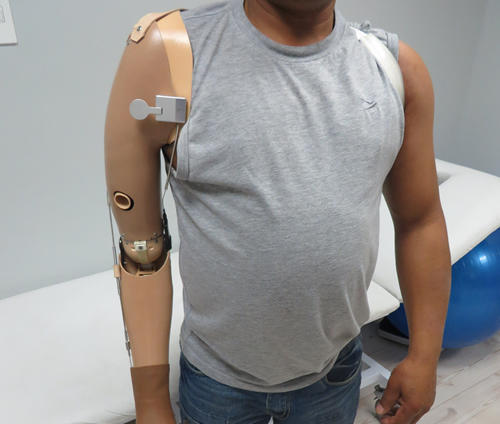
\includegraphics[width=10cm,height=7cm]{Figures/Contextual_figures/ProsthesesPics/above-elbow-prosthesis-500x500.jpg}
    \caption{A mechanical prosthesis operated by wire\cite{AEP}.}
    \label{fig:AEP}
\end{figure}
\subsection*{Electrical prostheses}
These prostheses have motors or actuators to move the joints of the prosthesis and can be used with different controllers and control systems. These prostheses are also the most expensive and advanced to use. Since the goal of the project is to provide as much support for the individual user, the electrical prosthesis is further explored. Some of the electrical prosthesis already on the market, e.g. the prosthesis in figure \ref{fig:DynaArm}.   
\begin{figure}[H]
    \centering
    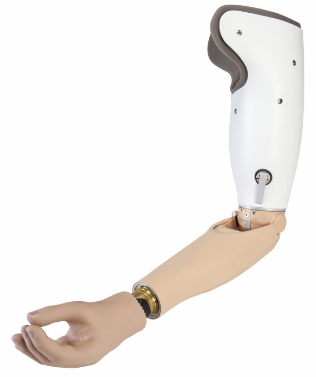
\includegraphics[width=6cm,height=6cm]{Figures/Contextual_figures/ProsthesesPics/dynamixarm.PNG}
    \caption{An Above elbow electrical prosthesis with DynamicArm from Ottobock\textsuperscript{\textcopyright} \cite{OttobockAB}}
    \label{fig:DynaArm}
\end{figure}
DynamicArm is a robotic prosthesis solution from Ottobock, this is for a person whom has had an amputation above the elbow joint. DynamicArm provides the user with the ability to flex the elbow joint\cite{OttobockAB}. The prosthesis can be used in combination with the Michelangelo hand which can rotate the wrist and utilise different grips\cite{OttobockM}. The prosthesis is used in combination with the Axon-Bus Prosthetic System, this bus system delivers a reliable source for data to the prosthesis and is safe for the user\cite{OttobockAX}.\\

\subsubsection*{Jaco}
Jaco is a stationary robotic manipulator. It is designed to be attached to a wheelchair operating as a left or right arm.\\
It weighs 5.2 kg, which makes it lightweight. The reach is 90 cm, and it utilises 6 degrees of freedom (D.O.F) It comes with a default joystick, that has many features, such as operating each joint of the arm and the fingers. Jaco can also initiate a "drinking mode", where it helps lifting the cup to drink from and rotate the wrist for the user to drink from the cup \cite{JACO}.\\
For a picture of the Jaco see figure \ref{fig:Sebastién}:
\begin{figure}[H]
    \centering
    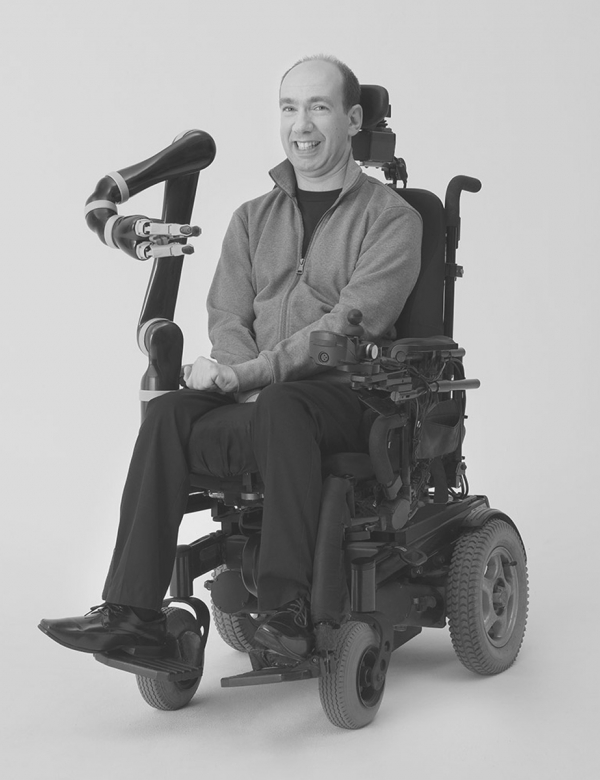
\includegraphics[width=7cm,height=7cm]{Figures/Technical_figures/Sebastien.jpg}
    \caption{Sabastién from Kinova with the Jaco arm on his wheelchair, All rights reserved to Kinova \ref{fig:KinovaPicture} \cite{Kinova}.}
    \label{fig:Sebastién}
\end{figure}
